\clearpage
\section{Methods}
\label{sec.methods}

Schema of the proposed method is illustrated in Fig.~\ref{fig.schema}. There are five major stages in this method, including 

\begin{figure}[!h]
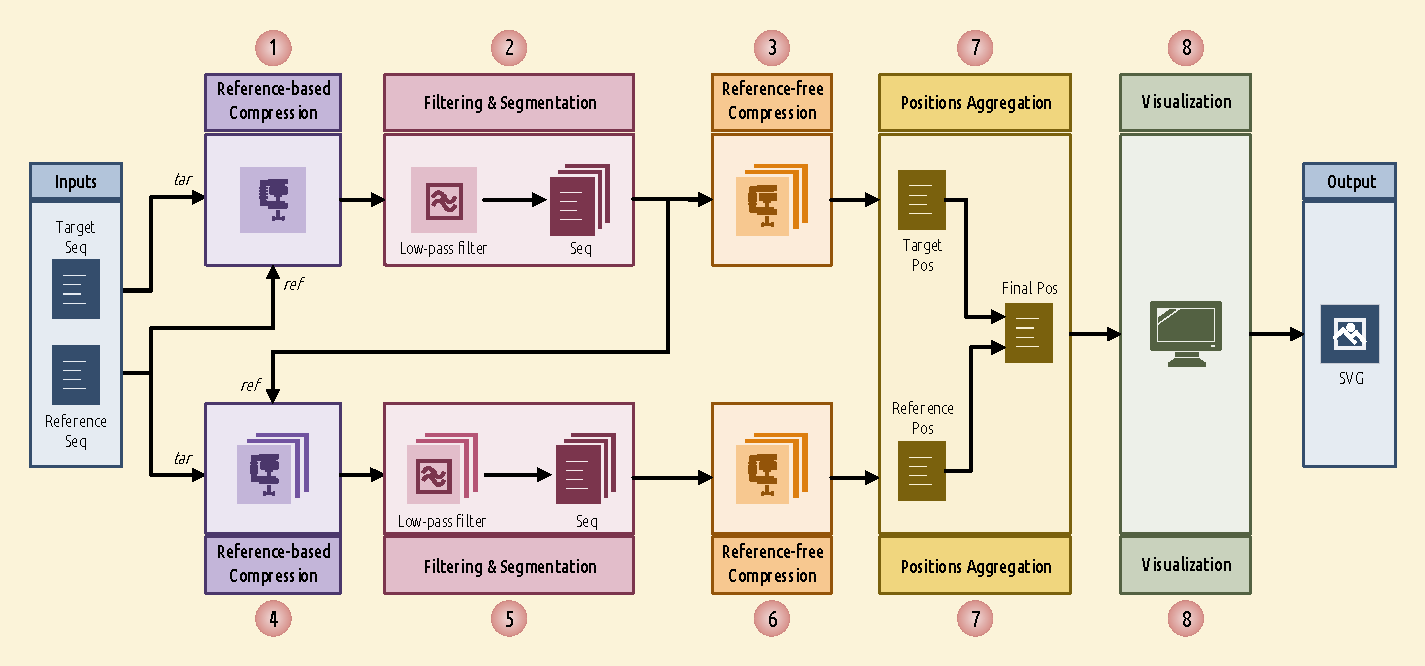
\includegraphics[width=\linewidth]{schema.pdf}
\caption{The schema of Smash++.}
\label{fig.schema}
\end{figure}

\subsection{Building models of the data}

\subsection{finding similar regions}

In order to smooth the profile information, we use Hann window, which is a discrete window function given by
\begin{equation}
  \label{eq.hann}
  w[n]=0.5\;\left[1-\cos \left({\frac {2\pi n}{N}}\right)\right]=\sin ^{2}\left({\frac {\pi n}{N}}\right),
\end{equation}
in which, $0\le n\le N$ and length of the window is $N+1$ (Fig.~\ref{fig.hann}).
\begin{figure}[!h]
  \centering
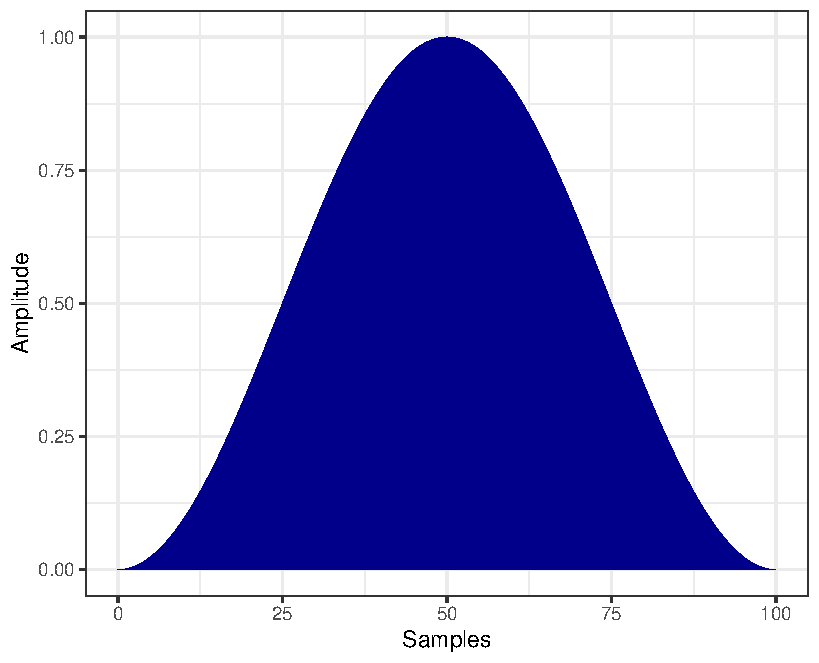
\includegraphics[width=7cm]{hann.pdf}
\caption{Hann window for 101 samples.}
\label{fig.hann}
\end{figure}

\subsection{Computing complexities}

\subsection{The software}

Besides Hann window, that is used as default to filter the profile information obtained by the reference-based compression, we have implemented several other window functions, shown in Fig.~\ref{fig.filters}.
\begin{figure}[!h]
  \centering
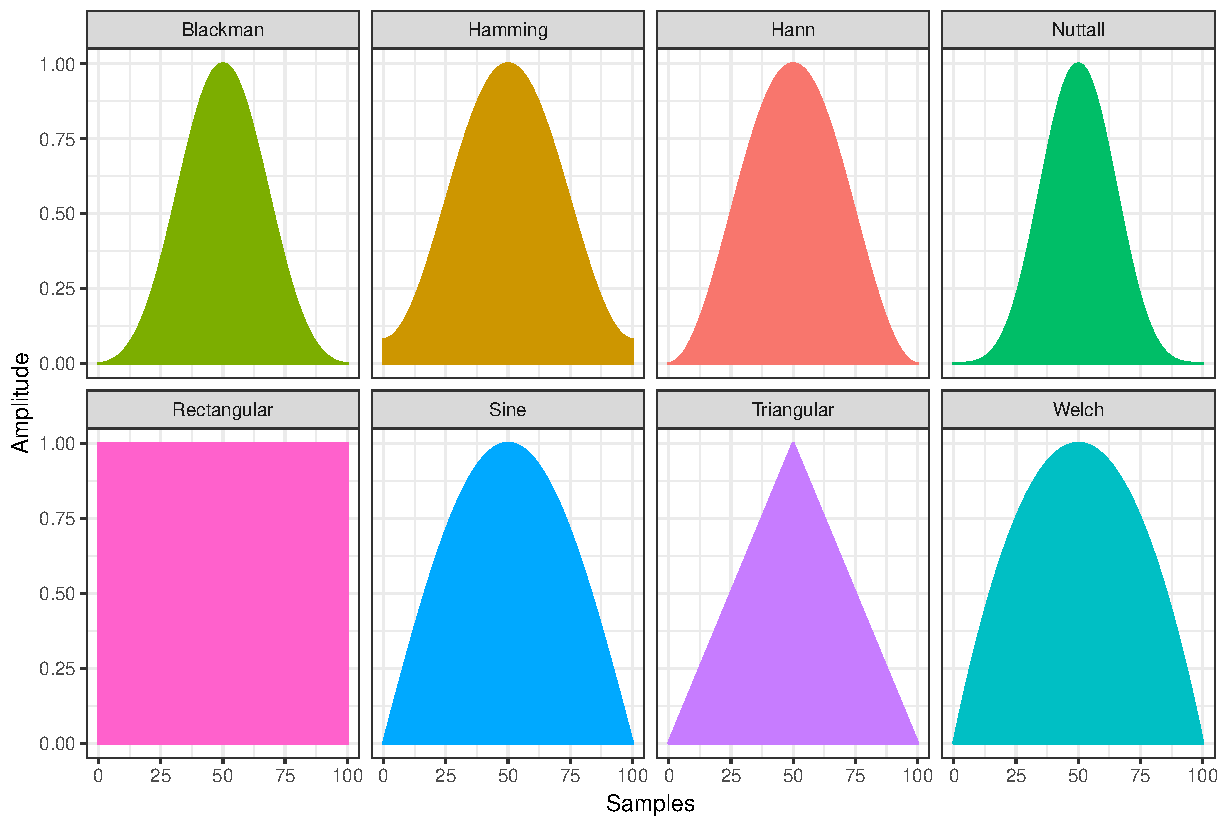
\includegraphics[width=.95\linewidth]{filters.pdf}
\caption{Window functions.}
\label{fig.filters}
\end{figure}
